\documentclass[utf8x]{beamer}
\usetheme{Frankfurt}
%\usetheme{Rochester}
\setbeamertemplate{navigation symbols}{}
\usepackage[ngerman]{babel}
\usepackage{listings}
\usepackage{tikz}

%\definecolor{hintergrundfarble}{rgb}{0.99,0.99,0.99}
\definecolor{colKeys}{rgb}{0,0,1}
\definecolor{colIdentifier}{rgb}{0,0,0}
\definecolor{colComments}{rgb}{1,0,0}
\definecolor{colString}{rgb}{0,0.5,0}
\lstset{
    language=c,
    float=hbp,
    basicstyle=\ttfamily\normalsize\mdseries,
    identifierstyle=\color{colIdentifier},
    keywordstyle=\color{colKeys},
    stringstyle=\color{colString},
    commentstyle=\color{colComments},
    columns=flexible,
    tabsize=4,
    frame=none, %single,
    extendedchars=false,
    showspaces=false,
    showstringspaces=false,
    numbers=none, %left,
  %  breaklines=true,
  %  backgroundcolor= \color{hintergrundfarble},
  %  breakautoindent=true
}

%\lstset{
%  emph={@Entity},         emphstyle=\color{red},
%  emph={@Id},             emphstyle=\color{red},
%  emph={@GeneratedValue}, emphstyle=\color{red},
%  emph={@OneToOne},       emphstyle=\color{red},
%  emph={@JoinColumn},     emphstyle=\color{red}
%}


\definecolor{darkblue}{rgb}{0,0,.5}
\definecolor{fh-blau}{rgb}{0.537255, 0.780392, 0.796078}
\definecolor{fh-gruen}{rgb}{0.364706, 0.658824, 0.172549}

\setbeamercolor{structure}{fg=fh-gruen}
\setbeamercolor{section in toc}{fg=black}
\setbeamercolor{subsection in toc}{parent=section in toc}

\title[libsnap]{\texttt{libsnap}}
\subtitle{Scaleable Node Address Protocol}
\author[Stefan B\"ohmann | sboehm@technik-emden.de]{Stefan B\"ohmann \newline \scriptsize \texttt{<sboehm@technik-emden.de>}}
\institute[FH Emden/Leer]{Fachhochschule Emden/Leer}
\logo{
\includegraphics[width=1cm,height=1cm]{images/logo_el_small.png}}
\titlegraphic{
\includegraphics[scale=0.2]{images/logo_el_small.png}}
\date{\today} 

\setbeamercovered{invisible}         %\setbeamercovered{transparent}

\begin{document}

\begin{frame}
    \thispagestyle{empty}
    \titlepage
    \vfill
    \begin{center}
        
\includegraphics[scale=0.25]{images/cc-by-white.png}\hspace*{0.2ex}
        
\includegraphics[scale=0.25]{images/cc-nc-white.png}\hspace*{0.2ex}
        
\includegraphics[scale=0.25]{images/cc-sa-white.png}
        \\\textcolor{red}{DRAFT}
        \\\tiny 
        Except where otherwise noted, this work is licensed under the Creative Commons
        \textit{\textcolor{darkblue}{\href{http://creativecommons.org/licenses/by-nc-sa/3.0}{Attribution-Noncommercial-Share~Alike}}} 3.0 License
        \vspace*{0.5ex}
    \end{center}
\end{frame}

\section{Einleitung}

\subsection{S.N.A.P}
\begin{frame}
\frametitle{S.N.A.P}
Protokollspezifikation der schwedischen Firma HTC.\\
Entwickelt f\"ur die Produktpalette der Hausautomatisierungssysteme rund um das
Power Line Modem \texttt{PLM-24}.
\end{frame}

\subsection{S.N.A.P Features}
\begin{frame}
\frametitle{S.N.A.P Features}
\begin{itemize}
  \item Easy to learn, use and implement
  \item Free and open network protocol
  \item<alert@2> Scaleable binary protocol with small overhead
  \item Up to 16.7 million node addresses
  \item Up to 24 protocol specific flags 
  \item<alert@3> Optional ACK/NAK request
  \item Optional command mode
  \item<alert@4> 8 different error detecting methods
  \item Media independent (power line, RF, TP, IR etc.)
  \item Works with simplex, half-, full- duplex links
  \item<alert@5> Header is scaleable from 3-12 bytes
  \item User specified number of preamble bytes (0-n)
  \item ...
\end{itemize}
\end{frame}

% kate: word-wrap off; encoding utf-8; indent-width 4; tab-width 4; line-numbers on; mixed-indent off; remove-trailing-space-save on; replace-tabs-save on; replace-tabs on; space-indent on;
% vim:set spell et sw=4 ts=4 nowrap cino=l1,cs,U1:

\section{libsnap}

\subsection{libsnap}
\begin{frame}

\only<1>{
  {\Huge \texttt{libsnap}}
}

\only<2->{
\begin{itemize}
  \item<2->freie Implementierung
  \begin{itemize}
    \item<2->GNU Lesser General Public License \textit{(LGPL)}
  \end{itemize}
  \item<3->Hardware- und Plattformunabhängig
  \begin{itemize}
    \item<3->geschrieben in C \textit{(C99, ISO/IEC 9899:1999)}
    \item<3->Buildsystem basiert auf CMake
  \end{itemize}
  \item<4->kleine Codebasis \textit{($\approx$ 3600 LOC)}
  \item<5->einheitliche, saubere API
  \item<6->keine dynamische Speicherallokierung
  \item<7->testgetriebenen Entwicklung
  \begin{itemize}
    \item<7->basiert auf dem CUnit Testing Framework
    \item<7->CTest - integriert im Build-Prozess
    \item<7->60\% Code sind Tests \textit{($\approx$ 2200 LOC)}
    \item<7->gcov/lcov basierter Coverage Report
    \item<7->dadurch $\approx$ 100\% Testabdeckung
  \end{itemize}
\end{itemize}
}
\end{frame}


\subsection{coverage}
\begin{frame}[fragile]
\begin{center}
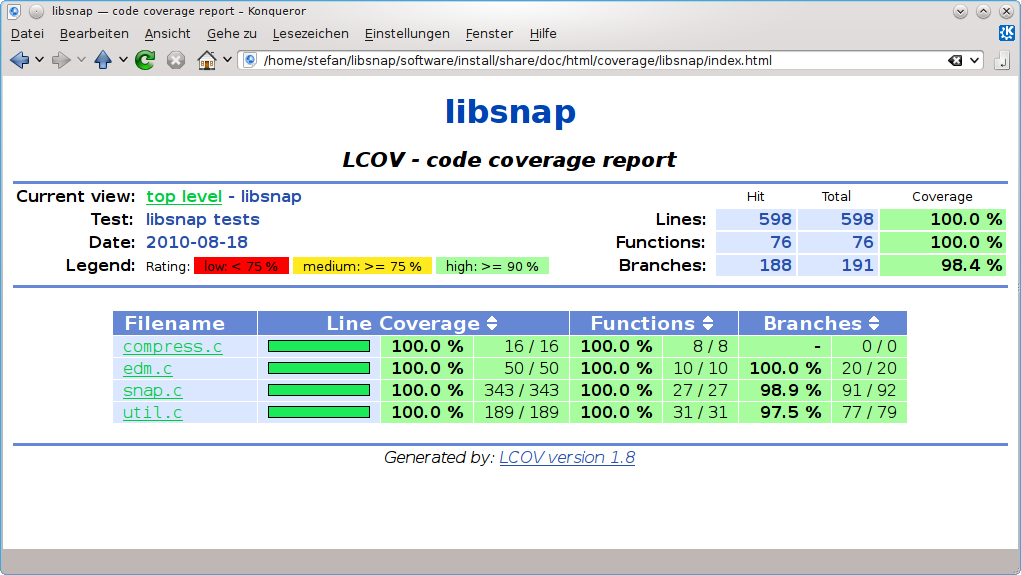
\includegraphics[scale=0.4]{images/lcov_1.png}
\end{center}
\end{frame}

\subsection{snap\_encode}
\begin{frame}[fragile]
\lstinputlisting[]{sources/encode.h}
\end{frame}


\subsection{snap\_encode\_bound}
\begin{frame}[fragile]
\lstinputlisting[]{sources/encode_bound.h}
\end{frame}


\subsection{snap\_decode}
\begin{frame}[fragile]
\lstinputlisting[]{sources/decode.h}
\end{frame}


\subsection{snap\_decode\_bound}
\begin{frame}[fragile]
\lstinputlisting[]{sources/decode_bound.h}
\end{frame}


\subsection{snap_example}
\begin{frame}[fragile]
\lstinputlisting[basicstyle =\ttfamily\footnotesize\mdseries]{sources/snap_example.c}
\end{frame}


\subsection{snap\_\ast}
\begin{frame}[fragile]
\lstinputlisting[basicstyle =\ttfamily\scriptsize\mdseries]{sources/snap_functions.h}
\end{frame}

\subsection{Issues}
\begin{frame}[fragile]
  \begin{itemize}
    \item<1->Das \texttt{EDM}-Flag kann unbemerkt kippen
    \item<2->Vorw\"artsfehlerkorrektur \texttt{FEC} wird erw\"ahnt, aber nicht spezifiziert
    \item<3->ein C-String wird ohne \texttt{NULL}-Terminierung dekodiert!
    \item<4->\texttt{encode} kann \"uber 100\% Overhead erzeugen
  \end{itemize}
\end{frame}
% kate: word-wrap off; encoding utf-8; indent-width 4; tab-width 4; line-numbers on; mixed-indent off; remove-trailing-space-save on; replace-tabs-save on; replace-tabs on; space-indent on;
% vim:set spell et sw=4 ts=4 nowrap cino=l1,cs,U1:

\section{libsnap++}

\subsection{libsnap++}
\begin{frame}[fragile]

\only<1>{
  {\Huge \texttt{libsnap++}}
}

\only<2->{
\begin{itemize}
  \item<2->libsnap f\"ur C++ Programmierer
  \item<3->sehr kleiner Wrapper \textit{($\approx$ 260 LOC)}
  \item<4->objektorientierte Schnittstelle
\end{itemize}
}
\end{frame}


\subsection{sourcecode1}
\begin{frame}[fragile]
\lstinputlisting[lang=c++]{sources/snap.cpp}
\end{frame}


% kate: word-wrap off; encoding utf-8; indent-width 4; tab-width 4; line-numbers on; mixed-indent off; remove-trailing-space-save on; replace-tabs-save on; replace-tabs on; space-indent on;
% vim:set spell et sw=4 ts=4 nowrap cino=l1,cs,U1:

\section{csnap}

\subsection{csnap}
\begin{frame}[fragile]
\only<1>{
  {\Huge \texttt{csnap}}\\
  CLI, Programmiersprache C, 650 LOC
}

\only<2>{
\begin{center}
 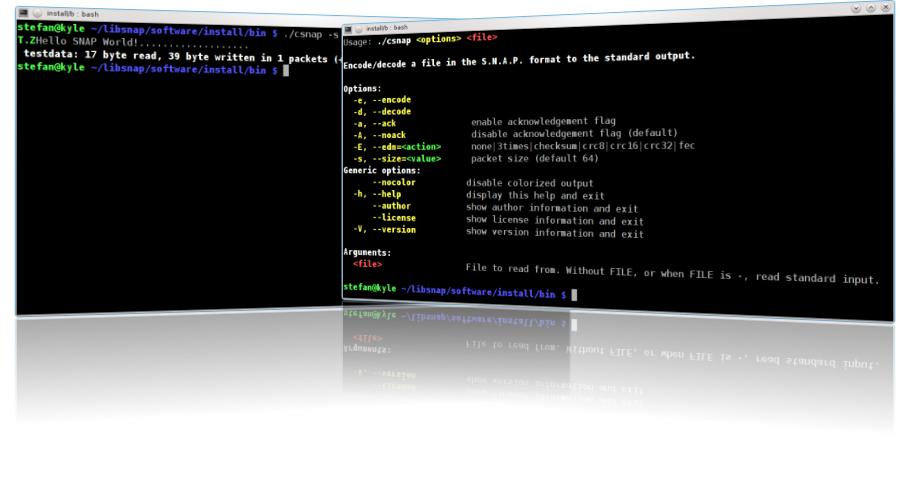
\includegraphics[scale=0.4]{images/screenie_csnap.png}
\end{center}
}
\end{frame}


\begin{frame}[fragile]
\begin{center}
 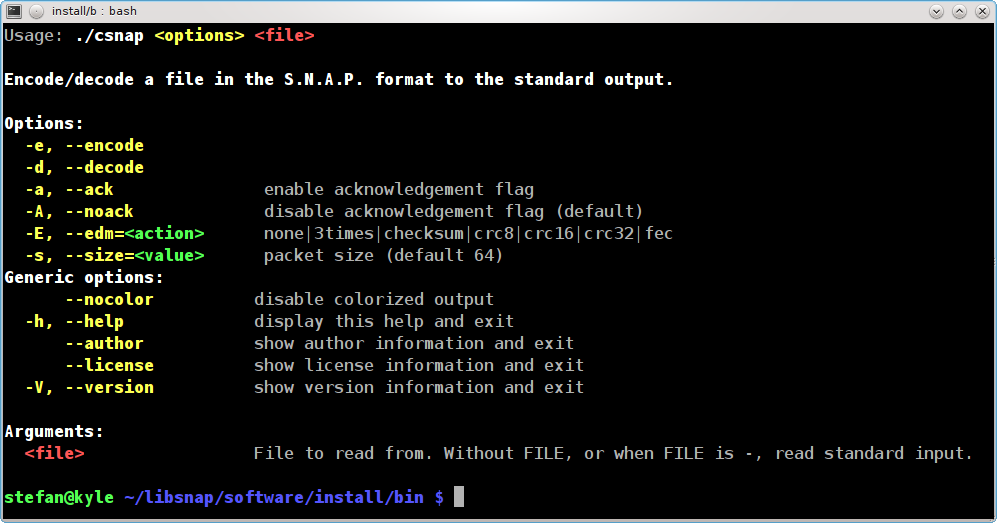
\includegraphics[scale=0.4]{images/csnap_1.png}
\end{center}
\end{frame}

\begin{frame}[fragile]
\begin{center}
 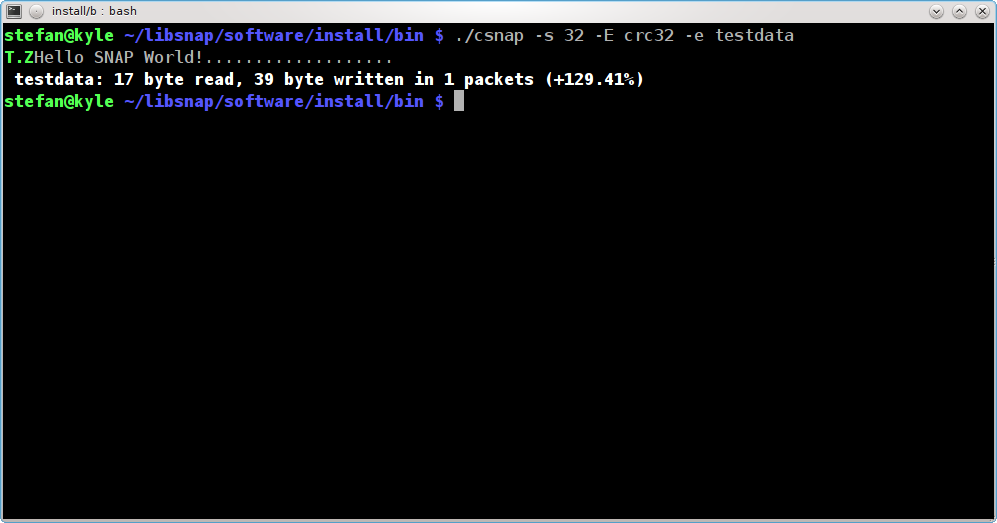
\includegraphics[scale=0.4]{images/csnap_2.png}
\end{center}
\end{frame}

\begin{frame}[fragile]
\begin{center}
 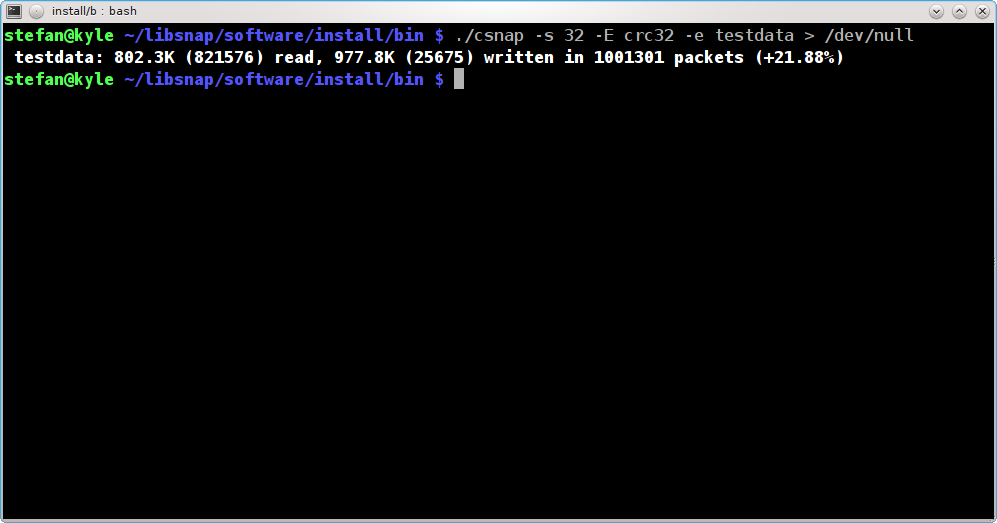
\includegraphics[scale=0.4]{images/csnap_3.png}
\end{center}
\end{frame}

% kate: word-wrap off; encoding utf-8; indent-width 4; tab-width 4; line-numbers on; mixed-indent off; remove-trailing-space-save on; replace-tabs-save on; replace-tabs on; space-indent on;
% vim:set spell et sw=4 ts=4 nowrap cino=l1,cs,U1:

\section{Utils}

\subsection{Utils}
\begin{frame}[fragile]
\only<1>{
  {\Huge \texttt{snapgauge}}\\
  GUI, Programmiersprache C++, 1500 LOC
}

\only<2>{
\begin{center}
 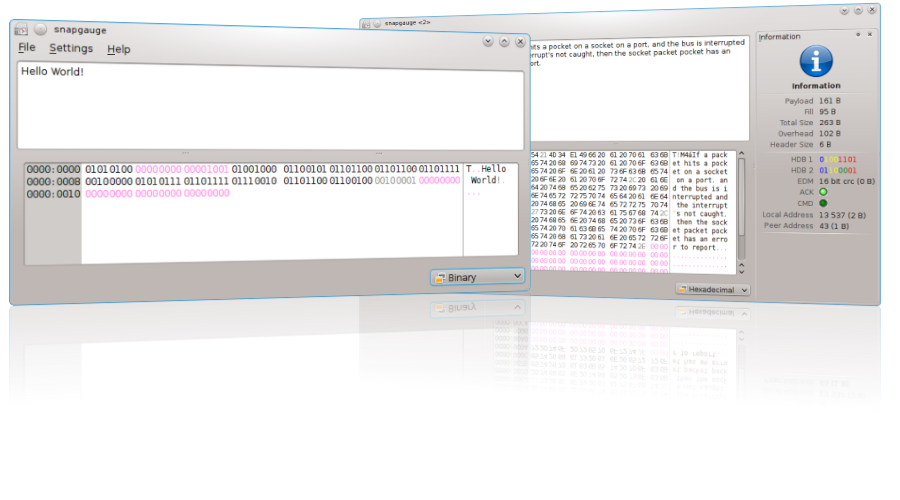
\includegraphics[scale=0.47]{images/screenie_snapgauge.png}
\end{center}
}
\end{frame}

\begin{frame}[fragile]
\begin{center}
 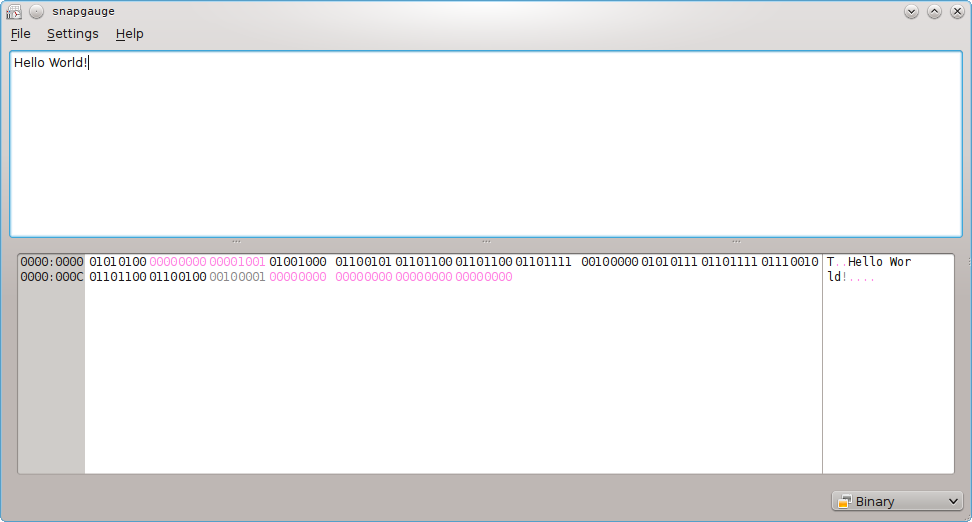
\includegraphics[scale=0.4]{images/snapgauge_1.png}
\end{center}
\end{frame}

\begin{frame}[fragile]
\begin{center}
 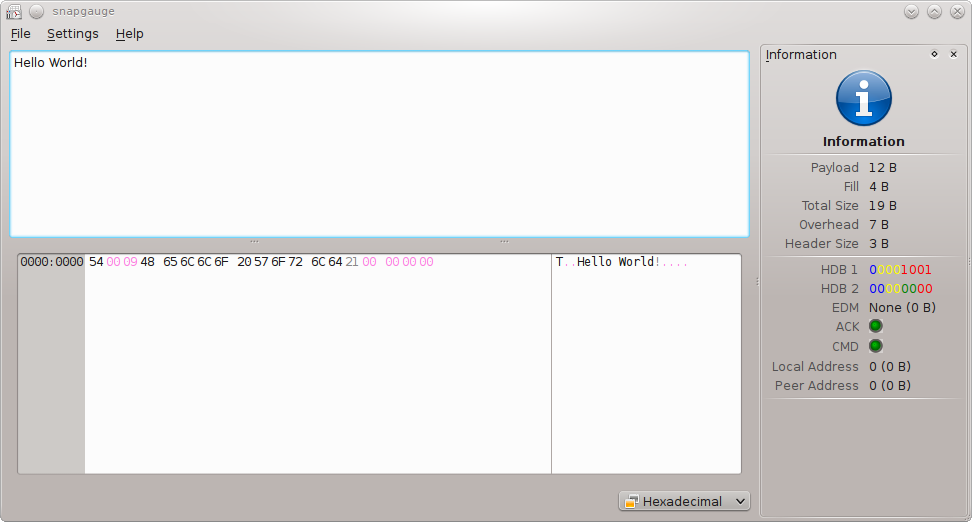
\includegraphics[scale=0.4]{images/snapgauge_2.png}
\end{center}
\end{frame}

\begin{frame}[fragile]
\begin{center}
 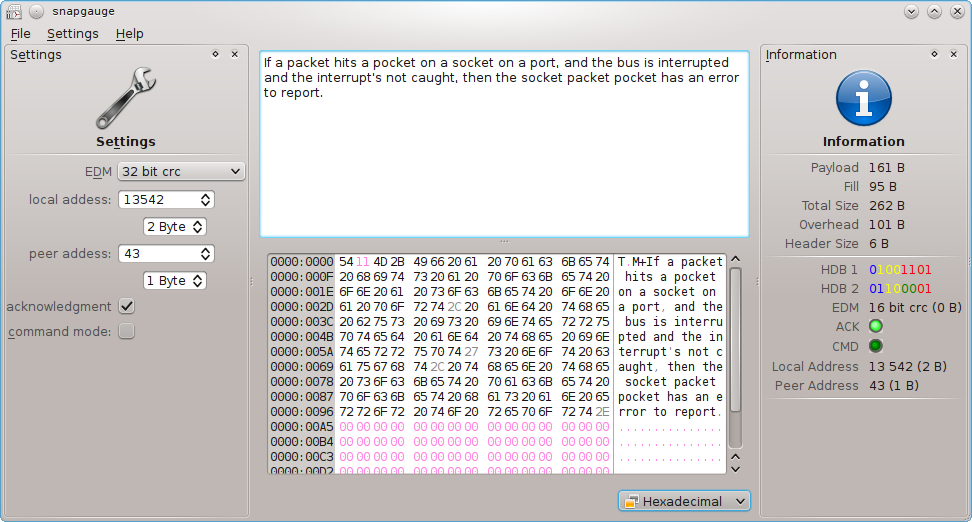
\includegraphics[scale=0.4]{images/snapgauge_3.png}
\end{center}
\end{frame}


% kate: word-wrap off; encoding utf-8; indent-width 4; tab-width 4; line-numbers on; mixed-indent off; remove-trailing-space-save on; replace-tabs-save on; replace-tabs on; space-indent on;
% vim:set spell et sw=4 ts=4 nowrap cino=l1,cs,U1:

\section{Fazit}
\subsection{Fazit}

\begin{frame}
\Huge
Fragen?
\end{frame}

\begin{frame}
\Huge
Thank you!

\end{frame}

% kate: word-wrap off; encoding utf-8; indent-width 4; tab-width 4; line-numbers on; mixed-indent off; remove-trailing-space-save on; replace-tabs-save on; replace-tabs on; space-indent on;
% vim:set spell et sw=4 ts=4 nowrap cino=l1,cs,U1:


\end{document}

% kate: word-wrap off; encoding utf-8; indent-width 4; tab-width 4; line-numbers on; mixed-indent off; remove-trailing-space-save on; replace-tabs-save on; replace-tabs on; space-indent on;
% vim:set spell et sw=4 ts=4 nowrap cino=l1,cs,U1:
